\documentclass[12pt,letterpaper]{article}
\usepackage{graphicx,textcomp}
\usepackage{natbib}
\usepackage{setspace}
\usepackage{fullpage}
\usepackage{color}
\usepackage[reqno]{amsmath}
\usepackage{amsthm}
\usepackage{fancyvrb}
\usepackage{amssymb,enumerate}
\usepackage[all]{xy}
\usepackage{endnotes}
\usepackage{lscape}
\newtheorem{com}{Comment}
\usepackage{float}
\usepackage{hyperref}
\newtheorem{lem} {Lemma}
\newtheorem{prop}{Proposition}
\newtheorem{thm}{Theorem}
\newtheorem{defn}{Definition}
\newtheorem{cor}{Corollary}
\newtheorem{obs}{Observation}
\usepackage[compact]{titlesec}
\usepackage{dcolumn}
\usepackage{tikz}
\usetikzlibrary{arrows}
\usepackage{multirow}
\usepackage{xcolor}
\newcolumntype{.}{D{.}{.}{-1}}
\newcolumntype{d}[1]{D{.}{.}{#1}}
\definecolor{light-gray}{gray}{0.65}
\usepackage{url}
\usepackage{listings}
\usepackage{color}
\usepackage{enumitem}


\definecolor{codegreen}{rgb}{0,0.6,0}
\definecolor{codegray}{rgb}{0.5,0.5,0.5}
\definecolor{codepurple}{rgb}{0.58,0,0.82}
\definecolor{backcolour}{rgb}{0.95,0.95,0.92}

\lstdefinestyle{mystyle}{
	backgroundcolor=\color{backcolour},   
	commentstyle=\color{codegreen},
	keywordstyle=\color{magenta},
	numberstyle=\tiny\color{codegray},
	stringstyle=\color{codepurple},
	basicstyle=\footnotesize,
	breakatwhitespace=false,         
	breaklines=true,                 
	captionpos=b,                    
	keepspaces=true,                 
	numbers=left,                    
	numbersep=5pt,                  
	showspaces=false,                
	showstringspaces=false,
	showtabs=false,                  
	tabsize=2
}
\lstset{style=mystyle}
\newcommand{\Sref}[1]{Section~\ref{#1}}
\newtheorem{hyp}{Hypothesis}

\title{Problem Set 1}
\date{Due: September 30, 2024}
\author{Applied Stats/Quant Methods 1}

\begin{document}
	\maketitle
	
	\section*{Instructions}
	\begin{itemize}
	\item Please show your work! You may lose points by simply writing in the answer. If the problem requires you to execute commands in \texttt{R}, please include the code you used to get your answers. Please also include the \texttt{.R} file that contains your code. If you are not sure if work needs to be shown for a particular problem, please ask.
\item Your homework should be submitted electronically on GitHub.
\item This problem set is due before 23:59 on Monday September 30, 2024. No late assignments will be accepted.
%\item Total available points for this homework is 80.
	\end{itemize}
	
	\vspace{1cm}
	\section*{Question 1: Education}

A school counselor was curious about the average of IQ of the students in her school and took a random sample of 25 students' IQ scores. The following is the data set:

\vspace{1cm}

\begin{enumerate}
	\item Find a 90\% confidence interval for the average student IQ in the school.\\
	
		
	\begin{enumerate}[label=(\alph*)]
		\item Find the Mean
		
			\lstinputlisting[language=R, firstline=48, lastline=48]{PS01_answersKBB.R}  			
		
		\item Find the Standard Error
					\lstinputlisting[language=R, firstline=51, lastline=51]{PS01_answersKBB.R}  
					
		\item Calculate the associated t-statistic using the degrees of freedom
					\lstinputlisting[language=R, firstline=53, lastline=57]{PS01_answersKBB.R}  
					
					
		\item Obtain the Upper and Lower Bounds
					\lstinputlisting[language=R, firstline=59, lastline=60]{PS01_answersKBB.R}  
					
					\lstinputlisting[language=R, firstline=61, lastline=62]{PS01_answersKBB.R}  
					
		\item This provides us with a confidence interval of:
		
		\textbf{ [93.960 , 102.920]} (3d.p)
	\end{enumerate}
	
	
	
	
	
	\item Next, the school counsellor was curious  whether  the average student IQ in her school is higher than the average IQ score (100) among all the schools in the country.\\ 
	
	\noindent Using the same sample, conduct the appropriate hypothesis test with $\alpha=0.05$.
	
	
	
\textbf{The 5 steps of Hypothesis Testing}
		\begin{enumerate}[label=(\alph*)]
	
		\item Assumptions\\
				We have assumed that the data is approximately normally distributed.\\
				We have also assumed that the IQ scores are independent of each other, as well as the sample being representative of the school.\\
				
		
		\item State $H_0$ and $H_a$\\
				
		Our $H_0$ is that the average IQ in her school is $ \leq $100.\\
		
		Our $H_a$ is that the average IQ in her school is $>$ 100\\
		
		

		
		\item Calculate the T-Statistic
	
			\lstinputlisting[language=R, firstline=74, lastline=76]{PS01_answersKBB.R}  
		
		\item Calculate the P-Value
			\lstinputlisting[language=R, firstline=81, lastline=82]{PS01_answersKBB.R}  

		\item Conclusion
		
		Given that the associated p-value is much larger than our significance level:
		$$0.721 > 0.05$$
		
		 We can say that there is \textbf{not} sufficient evidence for us to reject the null hypothesis. This suggests that there is no evidence to support the students having a higher IQ than the average (100) among all the schools in the country.
	
		\end{enumerate}
	
	
	
	
	
\end{enumerate}



\newpage

	\section*{Question 2: Political Economy}

\noindent Researchers are curious about what affects the amount of money communities spend on addressing homelessness. The following variables constitute our data set about social welfare expenditures in the USA. \\
\vspace{.5cm}


\begin{tabular}{r|l}
	\texttt{State} &\emph{50 states in US} \\
	\texttt{Y} & \emph{per capita expenditure on shelters/housing assistance in state}\\
	\texttt{X1} &\emph{per capita personal income in state} \\
	\texttt{X2} &  \emph{Number of residents per 100,000 that are "financially insecure" in state}\\
	\texttt{X3} &  \emph{Number of people per thousand residing in urban areas in state} \\
	\texttt{Region} &  \emph{1=Northeast, 2= North Central, 3= South, 4=West} \\
\end{tabular}

\vspace{.5cm}
\noindent Explore the \texttt{expenditure} data set and import data into \texttt{R}.
\vspace{.5cm}

\vspace{.5cm}

\begin{itemize}

\newpage
\item
Please plot the relationships among \emph{Y}, \emph{X1}, \emph{X2}, and \emph{X3}? What are the correlations among them (you just need to describe the graph and the relationships among them)?
\vspace{.5cm}
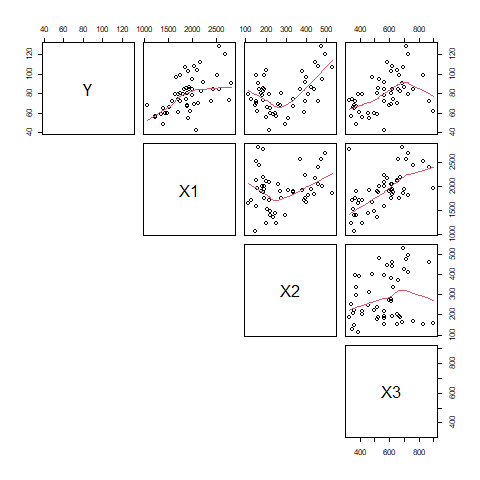
\includegraphics[width=0.8\textwidth]{images/pairs_plot.png}



X1,Y -  We see a slight positive correlation.\\
		This suggest there could be a positive relationship between state personal income per capita and state expenditure on housing assistance.\\
		

X2,Y - We see a non linear correlation.\\
		This implies the existence of some relationship between the number of financially insecure residence and state expenditure on housing assistance.\\
		

X3,Y - We observe no clear correlation.\\
		This suggests no relationship between the number of residents in urban areas and state expenditure on housing assistance.\\

X2,X1 - We see a slight non linear correlation.\\
		This implies the existence of some relationship between the number of financially insecure residence and state personal income per capita.\\

X3,X1 - We see a positive correlation.\\
		This suggest there could be a positive relationship between the number of residents in urban areas and state personal income per capita.\\
		
		 
X3,X2 - We observe no clear correlation.\\
		This suggests no relationship between the number of residents in urban areas and the number of financially insecure residence.\\



\newpage
\item
Please plot the relationship between \emph{Y} and \emph{Region}? On average, which region has the highest per capita expenditure on housing assistance?
\vspace{.5cm}

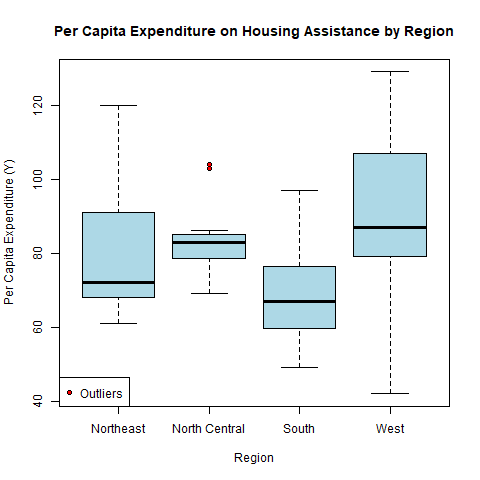
\includegraphics[width=0.8\textwidth]{images/Y_against_Region.png}

Looking at the box plot, we see on average (mean) the `West' region has the highest expenditure on housing assistance per capita, the box plot shows also that it has the largest range.

\newpage
\item
Please plot the relationship between \emph{Y} and \emph{X1}? Describe this graph and the relationship. Reproduce the above graph including one more variable \emph{Region} and display different regions with different types of symbols and colours.

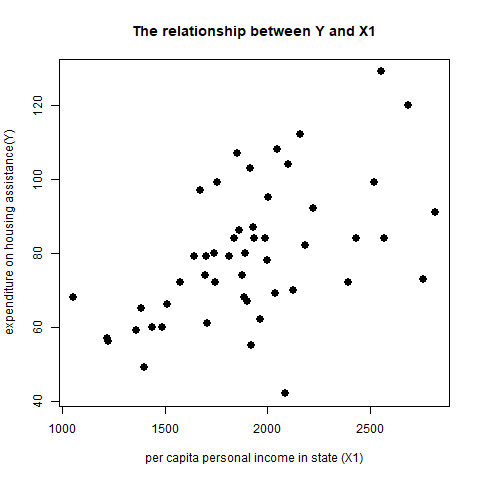
\includegraphics[width=0.5\textwidth]{images/Y_against_X1.png}
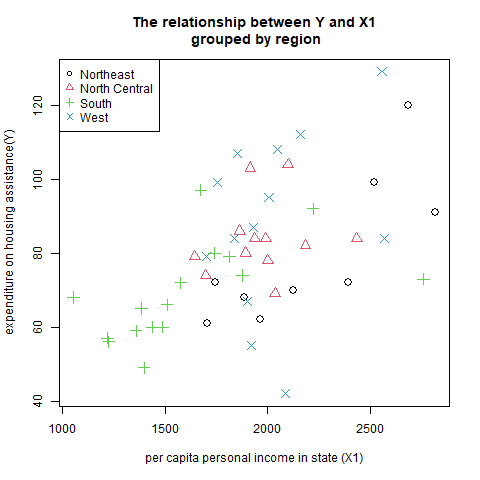
\includegraphics[width=0.5\textwidth]{images/Y_against_X1_with_legend.png}


Looking at the left hand graph we can see a general linear positive correlation between the two variables \textit{(X1 and Y)}.

However, when we split up the variables by region we see some different patterns emerge. For example looking at the `South' region we are able to identify the same positive correlation as before. But, when we observe the `West' and `North Central' regions this correlation is much less obvious.

Finally, upon observing the `Northeast' region, the two variables appear to have a non-linear relationship. With \textit{Y} climbing exponentially with minor increases \textit{X1}
\end{itemize}


\end{document}
